\RCS$Revision: 207461 $
\RCS$HeadURL: svn+ssh://snarayan@svn.cern.ch/reps/tdr2/notes/IN-14-XXX/trunk/IN-14-XXX.tex$
\RCS$Id: IN-14-XXX.tex 207461 2013-09-18 14:56:50Z tapper $
\newcommand{\Na}{N_\text{accesses}}
\newcommand{\Nf}{N_\text{files}}
\newcommand{\Nr}{\langle N_\text{rep}\rangle}
\newcommand{\fr}{f_\text{rep}^S}
\newlength\cmsFigWidth
\ifthenelse{\boolean{cms@external}}{\setlength\cmsFigWidth{0.85\columnwidth}}{\setlength\cmsFigWidth{0.4\textwidth}}
\ifthenelse{\boolean{cms@external}}{\providecommand{\cmsLeft}{top}}{\providecommand{\cmsLeft}{left}}
\ifthenelse{\boolean{cms@external}}{\providecommand{\cmsRight}{bottom}}{\providecommand{\cmsRight}{right}}
\input{commands.tex}
\cmsNoteHeader{IN 2014/XXX}

\title{Disk Storage Usage and Metrics for Dynamic Data Management}
\address[MIT]{Massachusetts Institute of Technology}
\author[MIT]{Y. Iiyama}
\author[MIT]{M. Goncharov}
\author[MIT]{S. Narayanan}
\author[MIT]{C. Paus}

\hypersetup{%
pdfauthor={M. Goncharov, Y. Iiyama, S. Narayanan, C. Paus},%
pdftitle={Disk Storage Usage and Metrics for Dynamic Data Management},%
pdfsubject={CMS},%
pdfkeywords={CMS, Dynamic Data Management, popularity}%
}

\date{\today}

\abstract{
%%
  In the CMS experiment, detector and Monte Carlo simulation data are ordered in
  datasets, which have some common properties and are usually analyzed as a
  whole.  The popularity of such datasets varies substantially, which opens the
  question how to best distribute the datasets such that they are optimally
  accessible at the various computing sites. Generally speaking, popular
  datasets should be replicated at several sites while less popular datasets
  might just have a single copy in the overall system. Also as the data taking
  progresses and new Monte Carlo simulation datasets become available, those
  datasets have to be distributed in the system and outdated datasets have to be
  removed. The Dynamic Data Management tools automatically manage the
  replication of datasets in the distributed multi-site computing system with
  the goal of optimising the system performance. In this note, we describe a
  metric for the performance of Dynamic Data Management, based on the number
  of user accesses of the given datasets.
%%
}

\maketitle %maketitle comes after all the front information has been supplied

\tableofcontents

%+++++++++++++++++++++++++++++++++++++++++++++++++++++++++++++++++++++++++++++++
\section{Introduction}\label{sec:introduction}

Dynamic Data Management currently manages a pool of approximately 80~PB across
several Tier-2 and Tier-1 sites. The purpose of the management to first order is
the creation and deletion of replicas of datasets that are part of the pool.
Additional replicas of a dataset are created when the dataset is particularly
popular, while excess replicas are deleted when they are less popular. The
creation and deletion of replicas does not add new datasets to the pool nor does
it remove datasets entirely from it. Adding new datasets to the pool and
completely removing datasets from it is treated separately. Newly created
datasets that are relevant to the Physics Group get automatically added to the
pool by the Computing Operations group and datasets will be deleted following
deletion campaigns that are driven by the Physics Groups in the experiment.
This means usually for a given dataset there is at least one copy in the system
often referred to as the last copy. If a dataset is declared deprecated, all
copies will be deleted.

A good measure of the performance of the algorithms used to create and delete
dataset replicas is the number of accesses per replica. If, for a given dataset,
this number is very large, then the dataset is not sufficiently replicated. On
the other hand, if it is very small for many datasets, then we are maintaining
too many replicas of unused datasets. To produce plots of the popularity of
datasets in a given time interval we have to carefully determine the list of
datasets that we have to consider and determine four attributes for each
dataset: number of accesses, size on disk, number of files, and average number
of replicas.

The plot provides a measure of how well our computing system is using the given
disk space in our data pool. In the following we explain in detail how we
determine the list of datasets we consider and how we calculate the four above
listed properties for each dataset.

%+++++++++++++++++++++++++++++++++++++++++++++++++++++++++++++++++++++++++++++++
\section{Ingredients}

%===============================================================================
\subsection{Dataset selection}

The CMS experiment creates a large number of datasets of which not all are
commonly used by the people doing analysis. These data tiers are mostly
stored on tape and are used for production purposes when the data or Monte Carlo
simulation samples get re-reconstructed with better calibrations/alignments
and/or new reconstruction algorithms. The majority of data on Tier 1 and Tier 2 
disks belong to the AOD, AODSIM, MINIAOD, and MINIAODSIM data tiers. In this study,
we restrict ourselves to datasets that have been assigned to the AnalysisOps 
PhEDEx group, for two reasons:
\begin{itemize}
  \item These subscriptions are created expressly for the purpose of user analysis,
    and therefore are the target of popularity-based replication and deletion.
  \item Production subscriptions (i.e. DataOps) are much shorter-lived, and furthermore,
    current estimates of popularity do not properly account for WMAgent accesses.
    Therefore, DataOps data appears completely unused, and it would be unfair to
    consider it as wasting disk space.
\end{itemize}

%===============================================================================
\subsection{Prorated disk usage}

PhEDEx directly provides us with the current locations of all datasets. However,
this information is not directly available for the past. Thus, PhEDEx transfer
and deletion histories are used to infer the timeline of the presence of a
dataset on a given site.

The histories are `sanitized' to remove self-inconsistent entries such as the
transfer of a dataset to a site on which it already exists. It is assumed that
each site can only contain one copy of a dataset. If there is no PhEDEx history
for a given dataset on a given site, but we know that the dataset is currently
on that site, then it is assumed to have existed on the site since its creation
time, which is determined using DBS.

First, we define the ``replica fraction'' as the fraction of the relevant time
interval that a particular replica existed at a site $S$:
%
\begin{equation}
  f_\textrm{rep}^{S} = \frac{\textrm{time on $S$ during $[t_0,t_1]$}}{t_1 - t_0}
\end{equation}

For a given dataset, we define the average number of replicas $\Nr$ by summing over 
the sites:
%
\begin{equation}
  \Nr = \sum_{S\in \text{sites}} f_\textrm{rep}^{S}
\end{equation}
%
This gives the average number of replicas of a dataset in a specific time
interval. If a dataset was not at the site for the entire considered time
interval the count is prorated with the fraction of time it was present in the
interval.

%===============================================================================
\subsection{Other dataset properties}

The remaining variables are relatively easily extracted from the Dynamo database,
which in turn gets the information from DBS ($N_\mathrm{files}$ and size) or popDB
($\Na$).
%+++++++++++++++++++++++++++++++++++++++++++++++++++++++++++++++++++++++++++++++
\section{Definition of metric}

The ``metric'', as opposed to being a number, is a histogram. There are two definitions
proposed, each showing a slightly different picture. It should be emphasized that
neither definition is incorrect; the reader can pick which to use based on what
they would like to show.

%===============================================================================
\subsection{Per-replica}

For each replica of a dataset at a site $S$, the $x$-value of the histogram is 
fixed at:
%
\begin{equation}
  \frac{\Na^S}{N_\mathrm{files}}
\end{equation}
%
The weight of each replica is:
\begin{equation}
  \mathrm{size} \times \fr
\end{equation}
That is, if a dataset with one file exists on site A for half of the time interval 
and is accessed once, and then moved to site B for the remainder of the time but 
never accessed, two entries would be made with equal weight (size/2): one at $0$ 
and another at $0.5$. The case of $\Na^S=0$ is treated specially: if the dataset
was created before the time interval in question, the replica is put in a separate
``0 old'' bin.
An example of such a plot is shown in Figure~\ref{fig:replicas}.

\begin{figure}[htpb]
  \begin{center}
    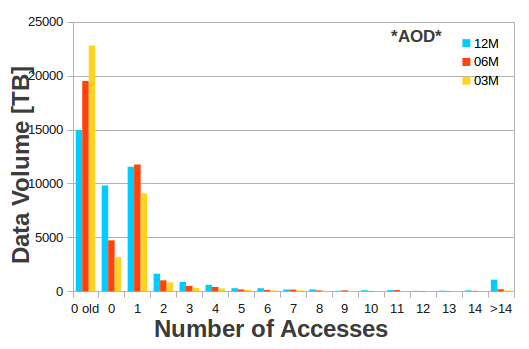
\includegraphics[width=0.85\textwidth]{plots/per_replica.png}
  \end{center}
  \caption{Popularity histogram filled with each replica treated separately.}  
  \label{fig:replicas}
\end{figure}


%===============================================================================
\subsection{Per-dataset}

For each dataset, the $x$-value of the histogram is fixed at:
%
\begin{equation}
  \frac{\sum_S\Na^S}{N_\mathrm{files}}
\end{equation}
%
The weight of each dataset is:
\begin{equation}
  \mathrm{size} \times \Nr
\end{equation}
That is, if a dataset with one file exists on site A for half of the time interval 
and is accessed once, and then moved to site B for the remainder of the time but 
never accessed, a single entry would be made with weight $2\times\mathrm{size}/2$ 
at $0.5$. Again, the case of $\Na^S=0$ is treated specially: if the dataset
was created before the time interval in question, it is put in a separate
``0 old'' bin.
An example of such a plot is shown in Figure~\ref{fig:datasets}.

\begin{figure}[htpb]
  \begin{center}
    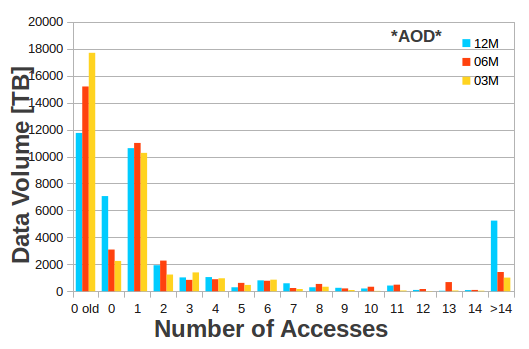
\includegraphics[width=0.85\textwidth]{plots/per_dataset.png}
  \end{center}
  \caption{Popularity histogram filled with each dataset as a single unit.}  
  \label{fig:datasets}
\end{figure}



\clearpage

%% **DO NOT REMOVE BIBLIOGRAPHY**
\bibliography{auto_generated}   % will be created by the tdr script.
%%% DO NOT ADD \end{document}!
